\begin{abstract}
Relative optical measurements depend on a reference, a collection geometry and the spectral response of the detector. We develop one reduction framework for RGBC counts, an LED-based relative sensor and an external analog UV detector. Example colour records distinguish selective response from saturation: all four RGBC channels clip at 4100 counts, while unsaturated filter extrema retain 0.872, 0.781 and 0.847 in their favoured channels after local referencing. A bracketed LED measurement gives a relative sample response of 0.553. The UV observations distinguish transmissions of 0.500, 0.400 and 0.283, with single-reading precision near 0.003 estimated from plateau scatter; their absolute irradiances use separate electrical and radiometric calibration factors. These comparisons identify what reference substitution cancels, which spectral and geometrical dependencies remain, and why small numerical scatter alone cannot establish an optical scale.
\end{abstract}
\begin{IEEEkeywords}
Relative photometry, spectral responsivity, transmission, reference substitution, UV radiometry, calibration.
\end{IEEEkeywords}

\section{One response model, different optical quantities}
A light sensor observes the radiation admitted by its aperture through a spectral response that is generally unequal to that of another detector. For a linearized indication $Y_k$, a useful model is
\begin{equation}
 Y_k=D_k+K_k\int s_k(\lambda)E_\lambda\,d\lambda+\epsilon_k,
 \label{eq:light-rgb-response}
\end{equation}
where $D_k$ is the offset, $K_k$ combines fixed gain and integration factors, $s_k$ is effective spectral responsivity and $E_\lambda$ is incident spectral irradiance. Changing a coloured scene changes $E_\lambda$. Inserting a filter replaces it by $E_\lambda\tau(\lambda)$, where $\tau$ is spectral transmission. Neither operation implies that the detector indication is illuminance or total radiant power.

Three acquisition paths make these distinctions concrete. The APDS-9960 on the original Nano 33 BLE Sense supplies clear, red, green and blue counts with overlapping spectral bands\cite{apds9960}. Puck.js uses an LED as a relative detector; LED photodetection is well established\cite{mims1992}, but its light function's 0--1 output has no absolute optical unit\cite{pucklight2026}. The UV path instead uses an external detector and signal conditioner feeding an analog input. Its optical band is determined by that detector, not by the board's RGB sensor.

Equation~\eqref{eq:light-rgb-response} relates the measured indication to incident irradiance. The Puck ratios compare relative response across the bracketed optical states; their interpretation as power ratios depends on response linearity. Multichannel-sensor calibration also requires separate treatment of spectral responsivity and absolute scale, as illustrated by Besozzi and colleagues for other compact detectors\cite{besozzi2026}. The examples considered here are separate optical comparisons; their response ratios cannot rank instrument accuracy or be treated as observations of one shared sample and spectrum.

\section{What reference substitution cancels}
Figure~\ref{fig:light-rgb-apparatus} fixes the source, aperture and detector while the sample or opaque stop is exchanged. Direct stray light that bypasses a sample does not follow its transmission, so baffling is part of the definition of the measurement. Reflection, scattering and fluorescence can also change which radiation reaches the detector. Reference spectrophotometry consequently specifies the collection geometry as well as the sample and reference\cite{BurkeMavrodineanu1983}.

\begin{figure}[!htbp]
\centering
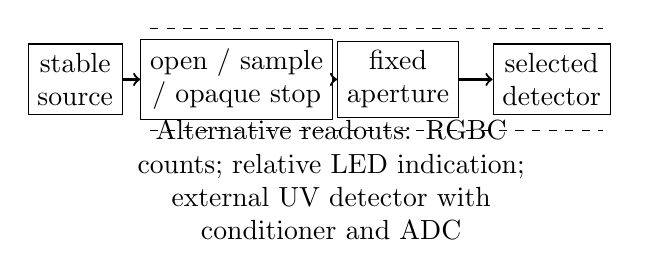
\begin{tikzpicture}[x=1cm,y=1cm]
 \node[draw,align=center] (s) at (.65,1) {stable\\source};
 \node[draw,align=center] (f) at (2.7,1) {open / sample\\/ opaque stop};
 \node[draw,align=center] (a) at (4.75,1) {fixed\\aperture};
 \node[draw,align=center] (d) at (6.7,1) {selected\\detector};
 \draw[->,thick] (s)--(f);\draw[->,thick] (f)--(a);\draw[->,thick] (a)--(d);
 \draw[dashed] (1.6,.35)--(7.35,.35);\draw[dashed] (1.6,1.65)--(7.35,1.65);
 \node[align=center,text width=7.1cm] at (3.9,-.28)
 {Alternative readouts: RGBC counts; relative LED indication;\\external UV detector with conditioner and ADC};
\end{tikzpicture}
\caption{Reference-substitution arrangement for each detector. A covered detector supplies the offset; the open path defines the reference. Source and detector geometry are held fixed as the sample or opaque stop is exchanged.}
\label{fig:light-rgb-apparatus}
\end{figure}

For sample, open-reference and dark indications $S$, $R$ and $D$, respectively, define
\begin{equation}
 T_w=\frac{S-D}{R-D},\qquad R>D.
 \label{eq:light-rgb-ratio}
\end{equation}
When the indication is proportional to incident power and the gain is unchanged, this becomes
\begin{equation}
 T_w=\frac{\int s(\lambda)E_\lambda\tau(\lambda)\,d\lambda}
 {\int s(\lambda)E_\lambda\,d\lambda}.
 \label{eq:light-rgb-weighting}
\end{equation}
Stable multiplicative gain cancels. The source spectrum and detector weighting remain. A spectrally neutral attenuator yields the same ideal ratio across detectors, whereas a coloured filter generally does not. Nor can three broad ratios uniquely recover an arbitrary transmission spectrum.

The reference must represent the same physical state apart from the sample. A dim-room baseline describes one illuminated scene; it is not automatically a covered-detector electronic dark. Interleaving open references and dark observations tests different aspects of stability. A changed open reference can reveal lamp or throughput drift, while a changed dark level is especially important when the sample signal is weak.

\section{Colour coordinates, selective attenuation and clipping}
The first RGBC example proceeds from a dim scene through white and coloured conditions to an overexposed interval. Its dim means over $[0,4)\unit{s}$ are 38.50, 10.41, 11.80 and 6.81 counts for clear, red, green and blue. For a stationary colour interval, a useful detector coordinate is
\begin{equation}
 p_k=\frac{\bar C_k-B_k}{\sum_{j\in\{R,G,B\}}(\bar C_j-B_j)},
 \qquad k\in\{R,G,B\},
 \label{eq:light-rgb-fractions}
\end{equation}
where $B_k$ is that dim-scene mean. The fractions sum to one; they describe relative changes from the starting scene rather than standard chromaticity. Table~\ref{tab:light-rgb-spectral} calculates them from channel means over interior windows. Averaging instantaneous fractions would be a different estimator.

The same table applies Eq.~\eqref{eq:light-rgb-ratio} to a separate filter sequence. Here the specified offsets are 3, 2, 2 and 1 counts, and the open-reference means over $[4.5,5.5)\unit{s}$ are 1824.55, 940.40, 1017.40 and 567.50 counts. Those observed means are used consistently as denominators. The filter sequence changes continuously, so the one-second windows around its extrema describe local transitions, not equilibrium filter plateaux.

\begin{table}[!htbp]
\caption{Dim-subtracted RGB fractions (upper group) and locally referenced filter transmissions (lower group). Fractions sum to one; each transmission uses its own channel reference. Time windows are half-open and in seconds.}
\label{tab:light-rgb-spectral}
\centering\footnotesize
\begin{tabular}{@{}lrrr@{}}\toprule
Condition/window & Red & Green & Blue\\\midrule
\multicolumn{4}{l}{Dim-subtracted colour fractions $p_k$}\\
White, 6--14 & .374 & .401 & .224\\
Red, 16--24 & .830 & .124 & .046\\
Green, 26--34 & .130 & .788 & .082\\
Blue, 36--44 & .100 & .135 & .765\\\midrule
\multicolumn{4}{l}{Locally referenced filter transmissions $T_k$}\\
14.5--15.5 & .872 & .238 & .162\\
24.5--25.5 & .224 & .781 & .245\\
34.5--35.5 & .169 & .212 & .847\\\bottomrule
\end{tabular}
\end{table}

Figure~\ref{fig:light-rgb-spectral} separates channel discrimination from saturation. The coloured intervals favour their corresponding channels, while white does not give equal fractions because both illumination and channel responsivities are unequal. During $[46,49)\unit{s}$, all four channels remain at 4100 counts. Their near-equal fractions then reflect lost information, and zero scatter reflects clipping. The nominal ceiling follows the pinned approximately $11.12\unit{ms}$ integration and $16\times$ gain configuration\cite{arduinoapds,apds9960}; the register's bit width does not define the usable optical range.

\begin{figure}[!htbp]
\centering\begin{tikzpicture}
\begin{groupplot}[group style={group size=1 by 2,vertical sep=1.35cm},
 width=0.96\columnwidth,height=3.5cm,grid=major,enlarge x limits=false,
 legend style={font=\scriptsize,at={(0.5,1.03)},anchor=south,legend columns=4,
 draw=none,fill=none,column sep=4pt},tick label style={font=\scriptsize}]
\nextgroupplot[ylabel={Counts ($10^3$)},xlabel={Colour-response time (s)},ymin=0,ymax=4.8]
\addplot[csgray,densely dotted,line width=.8pt] table[col sep=comma,x=c0,y expr={\thisrow{c1}/1000}] {data/light_plot_v1-2.csv};\addlegendentry{Clear}
\addplot[csred,solid,line width=.8pt] table[col sep=comma,x=c0,y expr={\thisrow{c2}/1000}] {data/light_plot_v1-2.csv};\addlegendentry{Red}
\addplot[csteal,dashed,line width=.8pt] table[col sep=comma,x=c0,y expr={\thisrow{c3}/1000}] {data/light_plot_v1-2.csv};\addlegendentry{Green}
\addplot[csblue,dashdotted,line width=.8pt] table[col sep=comma,x=c0,y expr={\thisrow{c4}/1000}] {data/light_plot_v1-2.csv};\addlegendentry{Blue}
\nextgroupplot[ylabel={Channel transmission},xlabel={Filter-response device time (s)},ymin=-.02,ymax=1.15]
\addplot[csred,solid,line width=.8pt] table[col sep=comma,x=c0,y=c2] {data/drafts/optics-rgb-local.csv};\addlegendentry{Red}
\addplot[csteal,dashed,line width=.8pt] table[col sep=comma,x=c0,y=c3] {data/drafts/optics-rgb-local.csv};\addlegendentry{Green}
\addplot[csblue,dashdotted,line width=.8pt] table[col sep=comma,x=c0,y=c4] {data/drafts/optics-rgb-local.csv};\addlegendentry{Blue}
\end{groupplot}
\end{tikzpicture}

\caption{Upper: raw clear and RGB counts, including the clipped interval. Lower: channel transmissions referenced to the open-window mean of a separate filter sequence. Each panel retains its own record time.}
\label{fig:light-rgb-spectral}
\end{figure}

Reference choice has a visible numerical effect. With the specified, rather than locally observed, reference counts of 1800, 900, 1050 and 620, the nominally open interval gives RGB ratios 1.045, 0.969 and 0.915. Its mismatch is channel dependent, so one common intensity rescaling cannot remove it. Re-referencing changes the blue extremum from 0.775 to 0.847. The later open-window ratios over $[44.5,45.5)\unit{s}$ are 1.007, 1.001 and 1.007. This close return is useful, but neighbouring transitions still contribute to both windows; their difference is not a unique estimate of lamp drift or sample-replacement uncertainty.

\section{Bracketing a scalar relative detector}
The LED example supplies a complementary test of the reference rather than another colour coordinate. The source and detector remain fixed while the path is blocked, opened, attenuated and reopened. Table~\ref{tab:light-rgb-brackets} uses half-open receive-time windows that exclude transitions. Equal weight is assigned to the two dark-window means and to the two open-window means; longer intervals are not implicitly given a larger calibration weight.

\begin{table}[!htbp]
\caption{Bracketed LED-detector response in relative units. Means and sample SDs summarize within-window levels and fluctuations.}
\label{tab:light-rgb-brackets}
\centering\footnotesize
\begin{tabular}{@{}lrr@{}}\toprule
Receive interval (s) & Mean & SD\\\midrule
Dark, 1--9 & .01935 & .01766\\
Open, 12--18 & .89762 & .02044\\
Sample, 24--36 & .50592 & .02315\\
Open, 42--48 & .89613 & .01441\\
Dark, 52--59 & .02467 & .01802\\\bottomrule
\end{tabular}
\end{table}

The bracketed estimates are $D=0.022010$ and $R=0.896878$, giving $T_w=0.553126$. The mean ratio calculated with fixed entered levels $D=0.02$ and $R=0.90$ is 0.552185. Their difference of 0.000941 is an estimator choice, rather than an additional physical attenuation. The open means differ by $-0.001492$ detector unit and the dark means by $+0.005317$. The dark change is small relative to the open-minus-dark span but increasingly consequential for weak sample signals.

There are 41 negative pre-gate ratios near the dark intervals. These are background-subtraction diagnostics, not negative physical transmission. Silently clipping them before estimating an offset would bias the retained indications upward. The transmission display may exclude nonphysical results while preserving the underlying observations for this check. The Puck's sampling setting is $4\unit{Hz}$, below its documented $5\unit{Hz}$ limit\cite{pucklight2026}; that setting does not establish a uniform delivered sequence.

Figure~\ref{fig:light-rgb-reference-transfer} retains the Puck's device-clock origin at $1000\unit{s}$. Its numerical windows use the separate receive clock. Regressing receive time against elapsed device time gives slope 0.999818 and an RMS residual of $2.24\unit{ms}$. This describes the relation between two example clocks, not either clock's absolute accuracy or a one-way transport latency. Bracketing stable states reduces the sensitivity of a mean ratio to such timing differences without making the clocks interchangeable.

\section{UV transmission and two stages of absolute calibration}
The external UV example exposes another distinction: the ratio in Eq.~\eqref{eq:light-rgb-ratio} can cancel electrical scale factors, while an irradiance in $\unit{W\,m^{-2}}$ requires them. First relate ADC indication $q$ to terminal voltage, then voltage to a specified irradiance:
\begin{align}
 U&=gq+c,\label{eq:light-rgb-adc}\\
 E&=k(U_s-U_D)=kg(q_s-D).
 \label{eq:light-rgb-radiometry}
\end{align}
A stable additive voltage offset cancels; uncertainty in $g$ and $k$ remains. Detector responsivity calibration needs a defined optical scale and spectral conditions\cite{larason2008}. Spectral mismatch, out-of-band response and geometry can remain even when an electrical calibration is satisfactory\cite{larason2001}. A broad-band filter ratio is also distinct from a biologically weighted UV protection factor\cite{cie220}.

\begin{figure}[!htbp]
\centering\begin{tikzpicture}
\begin{groupplot}[group style={group size=1 by 2,vertical sep=1.5cm},
 width=0.96\columnwidth,height=3.3cm,grid=major,enlarge x limits=false,
 legend style={font=\scriptsize,at={(0.5,1.03)},anchor=south,legend columns=2,
 draw=none,fill=none,column sep=4pt},tick label style={font=\scriptsize}]
\nextgroupplot[ylabel={LED response},xlabel={Puck device clock (s)},ymin=-.04,ymax=1.1]
\addplot[csblue,solid,line width=.8pt] table[col sep=comma,x=c1,y=c2] {data/drafts/puck-light.csv};
\nextgroupplot[ylabel={UV signal (counts)},xlabel={UV device time (s)},xmin=0,xmax=40,ymin=0,ymax=720]
\addplot[csblue,solid,line width=.8pt] table[col sep=comma,x=c0,y=c2] {data/drafts/uv-transmission_raw.csv};\addlegendentry{Continuous signal}
\addplot[csred,only marks,mark=*,mark size=1.7pt] table[col sep=comma,x=c10,y=c9] {data/drafts/uv-transmission_observations.csv};\addlegendentry{Paired observations}
\end{groupplot}
\end{tikzpicture}

\caption{Upper: bracketed LED response on the Puck device clock. Lower: continuous UV counts and paired observations on their device-time axis, showing agreement within three counts.}
\label{fig:light-rgb-reference-transfer}
\end{figure}

For the UV trace, dark and open means over $[1,4)$ and $[6,9)\unit{s}$ are 9.85 and 609.90 counts, with sample SDs 1.30 and 1.54 counts. Sample means over $[11,14)$, $[16,19)$ and $[21,24)\unit{s}$ are 310.05, 250.19 and 180.20 counts. The paired observations use $D=10$ and $R=610$ counts. Table~\ref{tab:light-rgb-uv} retains that observation estimator rather than replacing it silently with plateau means.

\begin{table}[!htbp]
\caption{UV transmission and irradiance calculated with the stated electrical and detector coefficients. $u_T$ is single-reading precision from plateau scatter; coefficient calibration uncertainties enter the irradiance budget.}
\label{tab:light-rgb-uv}
\centering\footnotesize
\begin{tabular}{@{}rrrr@{}}\toprule
$q_s$ (count) & $T_w$ & $u_T$ & $E$ (mW/m$^2$)\\\midrule
310 & .500 & .0030 & 9.68\\
250 & .400 & .0030 & 7.74\\
180 & .283 & .0030 & 5.48\\\bottomrule
\end{tabular}
\end{table}

The entered coefficients are $g=3.22580645\unit{mV/count}$, $c=0$ and $k=0.01\unit{W\,m^{-2}\,V^{-1}}$. The first equals the nominal $3.3\unit{V}$ endpoint divided by 1023, giving the nominal voltage-per-count scale used in the irradiance calculation. An external detector and conditioner must remain within the verified analog input range; the RGB sensor itself supplies no UV measurement.

Timestamp matching tests the observation association separately from the scale. At $12.477\unit{s}$ the paired value is 310 counts and the continuous signal is 309. At $27.505\unit{s}$ they are 310 and 313 counts. Across all six observation times, the largest discrepancy is three counts, equivalent to 0.005 in transmission for the 600-count denominator. The observations support plateau-level attenuation comparisons but not exact identity with individual continuous samples. The continuous record's approximately $50\unit{ms}$ median spacing does not resolve that value discrepancy.

\section{Precision, shared references and optical identifiability}
For independent single-reading uncertainties in sample, reference and dark indications, Eq.~\eqref{eq:light-rgb-ratio} gives
\begin{equation}
 u_T^2=\frac{u_S^2+T_w^2u_R^2+(T_w-1)^2u_D^2}{(R-D)^2}.
 \label{eq:light-rgb-uncertainty}
\end{equation}
This expression uses one dark uncertainty because the same estimate enters numerator and denominator. Reusing dark and reference observations across several samples introduces covariance between their ratios. Temporal correlation and positioning variation also prevent the number of readings from being treated automatically as the number of independent trials.

Using the UV plateau SDs as single-reading uncertainties gives approximately 0.0030 for the first three observations. This conditional precision excludes gain calibration, spectral mismatch and geometry. Independent ideal ADC rounding alone would contribute about 0.00059 to the first ratio. It is smaller than the observed fluctuation contribution; adding it again to the empirical SD would double-count the rounding already present in those fluctuations.

The RGB transition windows and Puck sample interval constrain different aspects of this budget. Variation through a deliberate filter transition cannot be assigned a stationary-transmission standard error. Likewise, dividing the Puck sample SD of 0.02315 by the square root of 48 does not by itself establish an uncertainty of the mean. Complete sample replacements, repeated brackets and block statistics at relevant timescales would distinguish source drift, temporal covariance and geometrical repeatability.

A neutral-attenuator test at several source levels assesses proportionality while holding spectral shape fixed. Repeating it with a second source spectrum tests transfer of the spectral weighting. These checks answer different questions from moving farther from a lamp, which can confound source geometry and detector nonlinearity. For RGB channels, retaining the full vector also prevents apparent brightness stability from concealing a colour change.

The common reduction thus supports several precise but different conclusions: an unsaturated colour coordinate, a detector-weighted filter ratio, a bracketed scalar indication and a UV irradiance evaluated with the stated calibration coefficients. Resolved spectra, molecular identification and absolute optical calibration involve spectral resolution, reference measurements and the detector response in addition to relative signal precision. Reference substitution becomes informative when these remaining dependencies are kept attached to the quantity being inferred.
